\documentclass[12pt,a4paper]{article}
\usepackage[T2A]{fontenc}
\usepackage[utf8]{inputenc}
\usepackage[russian]{babel}
\usepackage{amsmath,amssymb,amsfonts}
\usepackage{graphicx}
\usepackage{geometry}
\usepackage{hyperref}
\usepackage{caption}
\geometry{a4paper, margin=2.5cm}
\setlength{\parindent}{0pt}
\setlength{\parskip}{0.5em}
\title{Никель-водородный кольцар}
\author{А. Ю. Дроздов}
\date{}

\begin{document}
\maketitle

\begin{figure}[htbp]
\centering
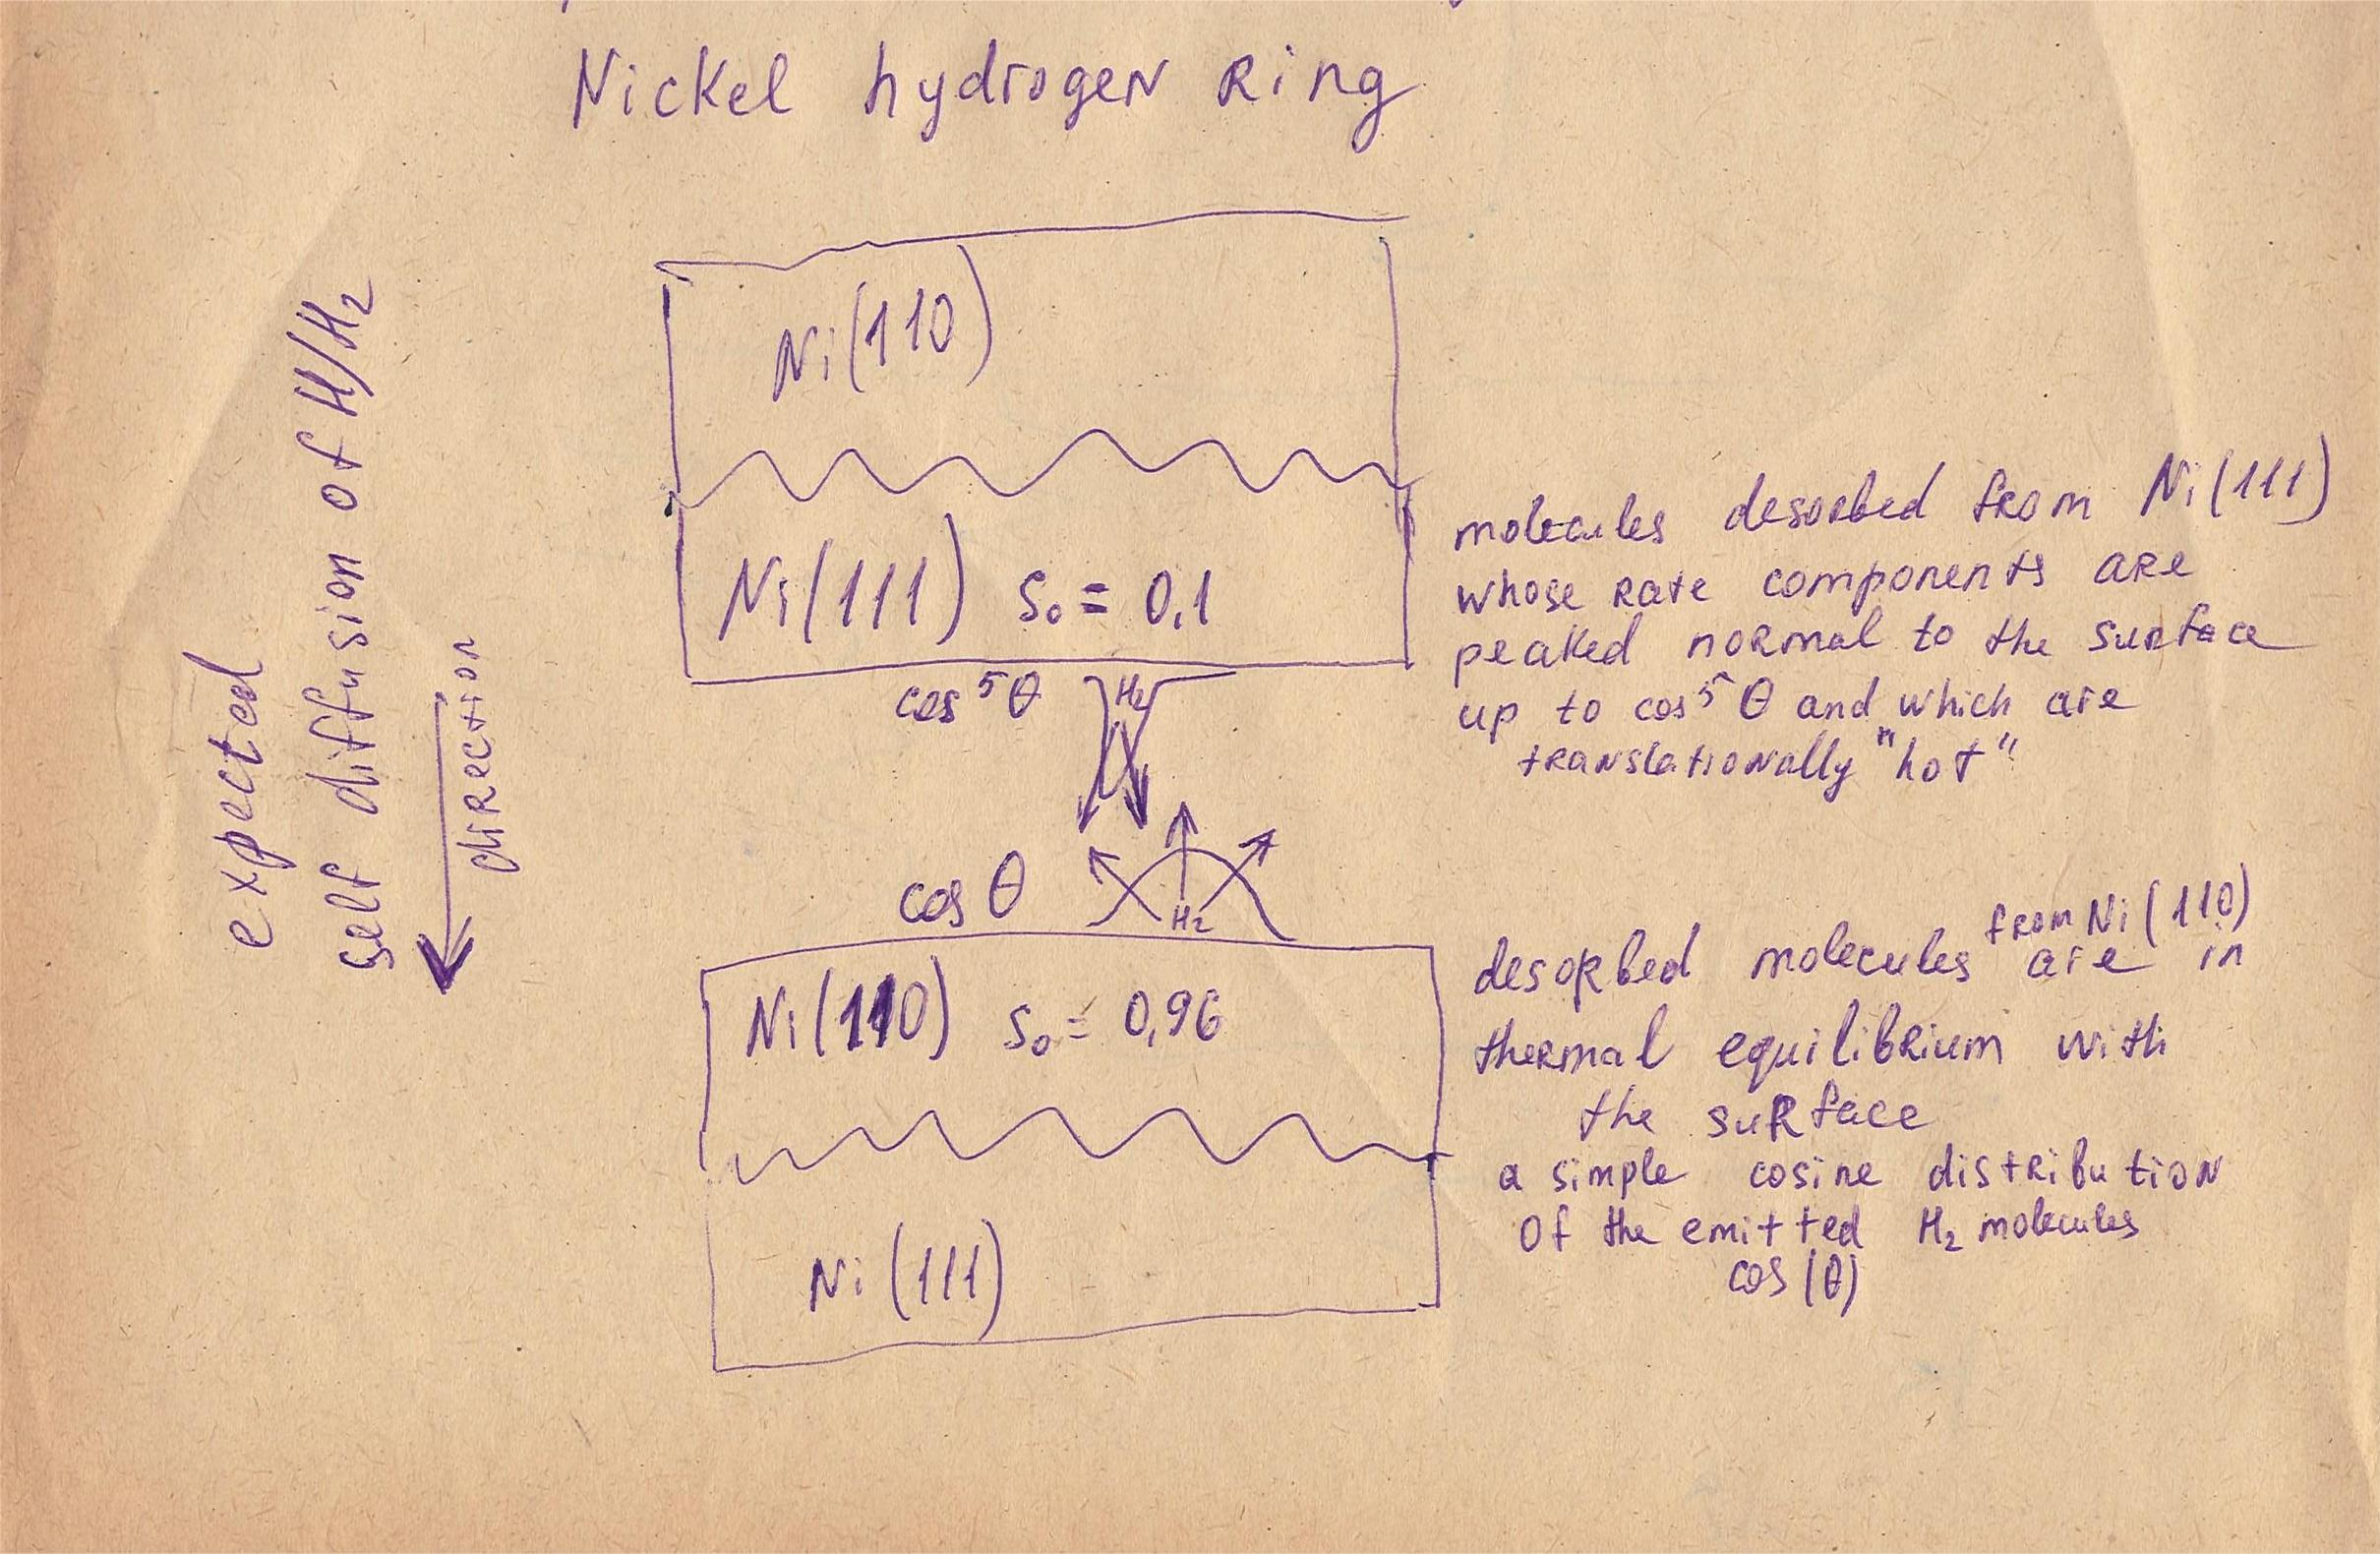
\includegraphics[width=0.8\textwidth]{Ni_H2_ring.jpg}
\caption{Схема никель-водородного кольцара}
\label{fig:ni_h2_ring}
\end{figure}

В данной работе рассматривается схема водородно-никелевого кольцара, ожидаемый эффект работы которого состоит в монотермическом превращении рассеянного тепла окружающей среды в механическую работу путем возникновения самопроизвольного устойчивого стационарного потока рабочего тела, которым является водород сквозь металлическую мембрану.

Идея была сформулирована с использованием теоретической информации изложенной в Christmann K. Interaction of hydrogen with solid surfaces // Surf. Sci. Rep. 1988. Vol. 9. P. 1--163 [ \url{https://doi.org/10.1016/0167-5729(88)90009-X} ].

Мой конспект этой работы с моими комментариями см. по ссылке: \url{https://nbviewer.org/github/daju1/articles/blob/master/perpetuum_mobile_of_the_second_kind/hydrogen_metal_membrane/iteraction_of_hydrogen_with_solid_surfaces.ipynb}

\section{Формула потока через мембрану}

Далее в работе 35. Nishimura C., Komaki M., Amano M. Hydrogen permeation characteristics of vanadium-nickel alloys // Mater. Trans. 1991. Vol. 32(5). P. 501--507 [\url{https://doi.org/10.2320/matertrans1989.32.501}].

приводится формула для потока через мембрану

\[
J = \Phi \left(P_u^{1/2} - P_d^{1/2} \right) \big / L
\]

где:
\begin{itemize}
    \item $J$ -- steady state hydrogen flux $\left(\text{mol}\, H_2 / (\text{m}^2 \cdot \text{s})\right)$
    \item $\Phi$ -- hydrogen permeability $\left(\text{mol}\, H_2 / (\text{m} \cdot \text{s} \cdot \text{Pa}^{1/2})\right)$
    \item $P_u, P_d$ -- hydrogen pressures at the upstream side and the downstream side (Pa)
    \item $L$ -- толщина мембраны (м)
\end{itemize}

В этой же работе приводится график:

\begin{figure}[htbp]
\centering
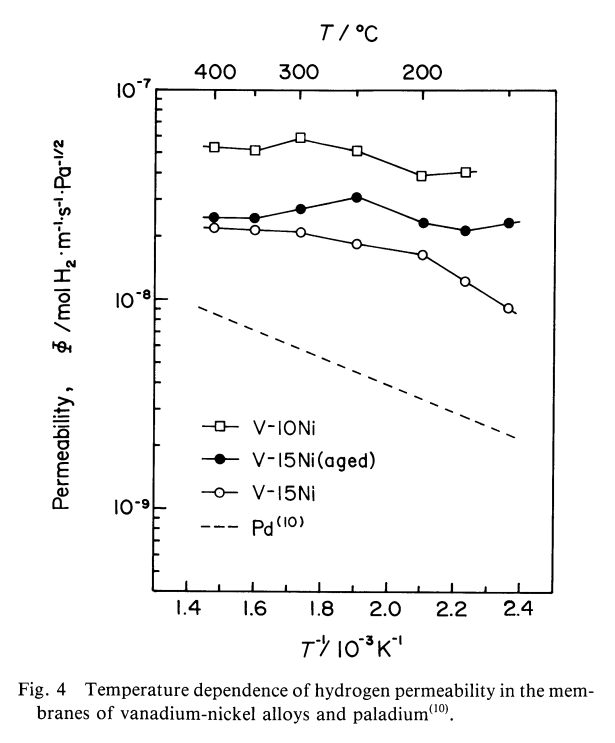
\includegraphics[width=0.8\textwidth]{nishimura1991_fig4.png}
\caption{График проницаемости водородных сплавов (Nishimura et al., 1991)}
\label{fig:nishimura}
\end{figure}

Из этого графика для температуры $T = 35 ^\circ \text{C} = 308 \text{ K}$ для палладиевой мембраны

\[
\Phi = 8 \cdot 10^{-9} \text{ mol}\, H_2 \cdot \text{m}^{-1} \cdot \text{s}^{-1} \cdot \text{Pa}^{-1/2}
\]

для мембраны из сплава ванадия с 10 \% никеля

\[
\Phi = 5 \cdot 10^{-8} \text{ mol}\, H_2 \cdot \text{m}^{-1} \cdot \text{s}^{-1} \cdot \text{Pa}^{-1/2}
\]

\section{Расчет потока и скорости газа}

Примем давления:
\[
p_{Pd(111)} = 7.94 \cdot 10^{-7} \text{ Torr} = 0.0001056 \text{ Pa}
\]
\[
\sqrt{p_{Pd(111)}} = 0.010278 \text{ Pa}^{-1/2}
\]

Вычислим поток:
\[
J_{V\_10Ni} = \Phi_{V\_10Ni} \frac{\sqrt{p_{Pt}} - \sqrt{p_{Pd}}}{L}
\]

При заданных параметрах ($L = 100 \cdot 10^{-6}$ м, $R = 8.31446262$ Дж/(моль·К), $T = 306.5$ К):

\[
J_{V\_10Ni} \approx 5.457 \cdot 10^{-5} \text{ mol}/(\text{m}^2\cdot\text{s})
\]

Допустим, что установление потока в 4 раза уменьшит величину $P_{Pd}$ и в столько же раз увеличит величину $P_{Pt}$. Тогда скорректированный поток:

\[
J = \Phi_{V\_10Ni} \frac{\sqrt{p_{Pt\_k}} - \sqrt{p_{Pd\_k}}}{L}
\]

Скорость потока в газовой фазе в метрах в секунду:

\[
v = \frac{J}{c} = J \frac{R T}{p}
\]

Получаем скорости на разных сторонах мембраны и расчетную удельную мощность по формуле, аналогичной оной в работе ``жидкокристаллический осмос'' (\url{https://nbviewer.org/github/daju1/articles/blob/master/liquidcrystalosmos/liquidcrystalosmos.ipynb}):

\[
w = \eta \cdot p \cdot V_{\text{ос}} \quad [\text{Вт}/\text{м}^2]
\]

\section{Десорбция как дифракция волн де Бройля молекул водорода на кристаллической решётке}

А вот на нижней по рисунку поверхности Ni(110) направленные наклонно к поверхности молекулы водорода будут достаточно эффективно адсорбироваться из-за достаточно широкого углового распределения $\cos(\theta)$ каналов адсорбции-десорбции на поверхности Ni(110).

Таким образом, в никель-водородном кольцаре именно зазоры могут выступать тем пространством, в котором можно ожидать нарушения принципа детального равновесия.

\section{Вычисление потока по модели десорбции}

Формула для плотности газа при десорбции:

\[
s_0 \bar{c} n_g = \nu_2 (\Theta) \, \exp \left(-\frac{\Delta E^{*}_{d} (\Theta)}{kT} \right) n_{ad}^2
\]

Отсюда плотность газа:

\[
n_g = \frac{\nu_2 (\Theta)}{s_0} \, \exp \left(-\frac{\Delta E^{*}_{d} (\Theta)}{kT} \right) \frac{n_{ad}^2}{\bar{c}}
\]

Параметры для разных граней палладия:
\begin{center}
\begin{tabular}{cccc}
Metal (hkl) & $\nu_2$ $\left(\frac{\text{cm}^2}{\text{s}\cdot\text{at}}\right)$ & $s_0$ & $\Delta E^{*}_{d}$ (кДж/моль) \\
Pd(100) & $23$ & $0.5$ & $96.6$ \\
Pd(110) & $23$ & $0.7$ & $96.6$ \\
\end{tabular}
\end{center}

При $R = 8.314$, $T = 300$ К, $n_s = 1.8 \cdot 10^{15}$ см$^{-2}$:

\[
n_g(100) \approx 6.27 \cdot 10^{10} \text{ м}^{-3}
\]
\[
n_g(110) \approx 5.60 \cdot 10^{12} \text{ м}^{-3}
\]

\section{Обсуждение технологических аспектов}

К сожалению, мне пока не известны экспериментальные данные, как будет атомарный водород преодолевать спай монокристаллов пусть даже одного металла, но с разными $hkl$. Теоретически этот спай будет зоной дефектов кристаллической структуры. Но если в этой зоне не будет какой-либо заметной примеси окислов, то какого-то большого барьера быть не должно.

Коэффициент диффузии для кристаллов как известно зависит от направления. Вследствие анизотропии свойств этого кристалла.

А вот если бы удалось создать такой монокристалл, у которого бы периодические барьеры активации процесса диффузии того же атомарного водорода также обладали бы свойством несимметричной деформируемости, но это был бы уже высший пилотаж.

\begin{figure}[htbp]
\centering
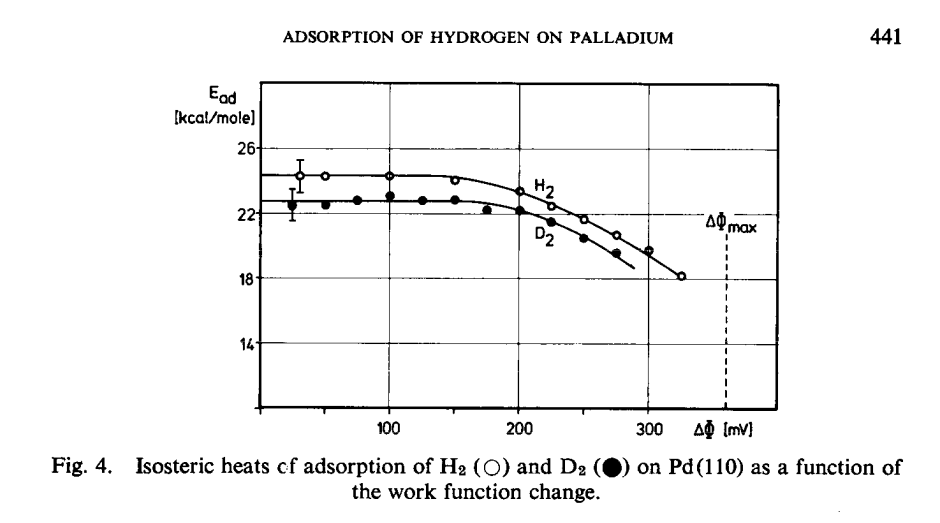
\includegraphics[width=0.7\textwidth]{conrad1974_fig4.png}
\caption{Изотермы адсорбции водорода на палладии (Conrad et al.)}
\label{fig:conrad4}
\end{figure}

\begin{figure}[htbp]
\centering
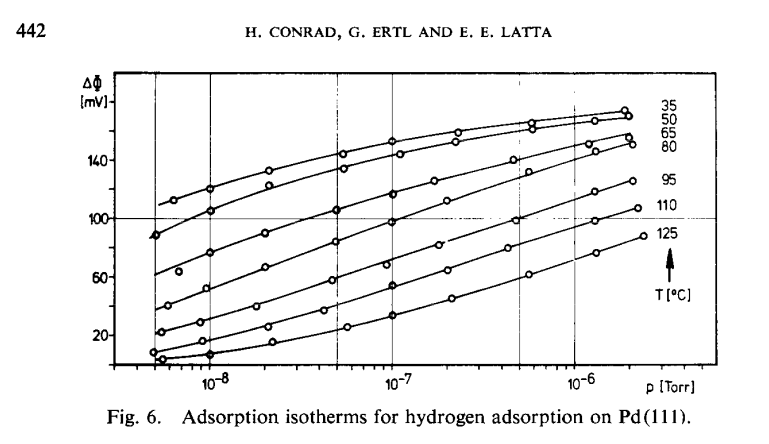
\includegraphics[width=0.7\textwidth]{conrad1974_fig6.png}
\caption{Температурная зависимость проницаемости (Conrad et al.)}
\label{fig:conrad6}
\end{figure}

\begin{figure}[htbp]
\centering
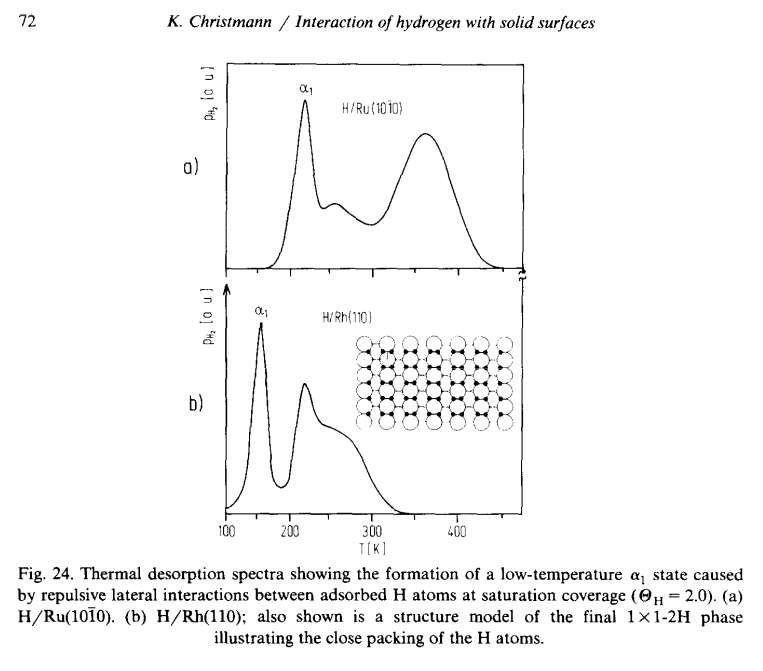
\includegraphics[width=0.7\textwidth]{Christmann_fig24.png}
\caption{Спектр термодесорбции водорода (Christmann)}
\label{fig:christmann}
\end{figure}

\section{Физико-химическое происхождение сверхпроницаемости}

Следует отметить крупномасштабное влияние химии поверхности на проницаемость и поглощение ``горячего'' водорода в металлах. См. работу: Livshits A. I., Notkin M. E., Samartsev A. A. Physico-Chemical Origin of Superpermeability-Large-Scale Effects of Surface Chemistry on ``Hot'' Hydrogen Permeation and Absorption in Metals // J. Nucl. Mater. 1990. Vol. 170, N 1. P. 79--94 [\url{https://doi.org/10.1016/0022-3115(90)90329-L}].

В разделе 2.4. Non-symmetric membranes рассматриваются несимметричные мембраны.

Мой конспект этой работы с критическими комментариями см. по ссылке: \url{https://nbviewer.org/github/daju1/articles/blob/master/perpetuum_mobile_of_the_second_kind/hydrogen_metal_membrane/sticking_of_hydrogen_to_Nb_containing_oxygen.ipynb}

\begin{figure}[htbp]
\centering
\includegraphics[width=0.6\textwidth]{VFK.jpg}
\caption{Схема вакуумно-фотокаталитического кольцара (аналогия)}
\label{fig:vfk}
\end{figure}

\section{Известные аналогии}

\begin{itemize}
    \item Электрофизический кольцар Жвирблиса
    \item Найквистор Виноградова
    \item Жидкокристаллический осмос
    \item Неэрмитовые квантовые системы Тимофеева и Колотинского
\end{itemize}

Рассматривая идею статьи Тимофеева-Колотинского о том, что для неэрмитовых систем получаются локальные отклонения как от 3 закона Ньютона, так и от 2 начала термодинамики.

Так как на самом деле на кинетику диффузии водорода будут в значительной мере влиять явления дифракции, которые со своей стороны зависят от ориентации $hkl$ кристалла. Поэтому одномерная постановка задачи, которая рассматривается в теоретических работах, это лишь некоторое первое приближение, не учитывающее трехмерных ориентационных эффектов кристаллической решетки.

\begin{figure}[htbp]
\centering
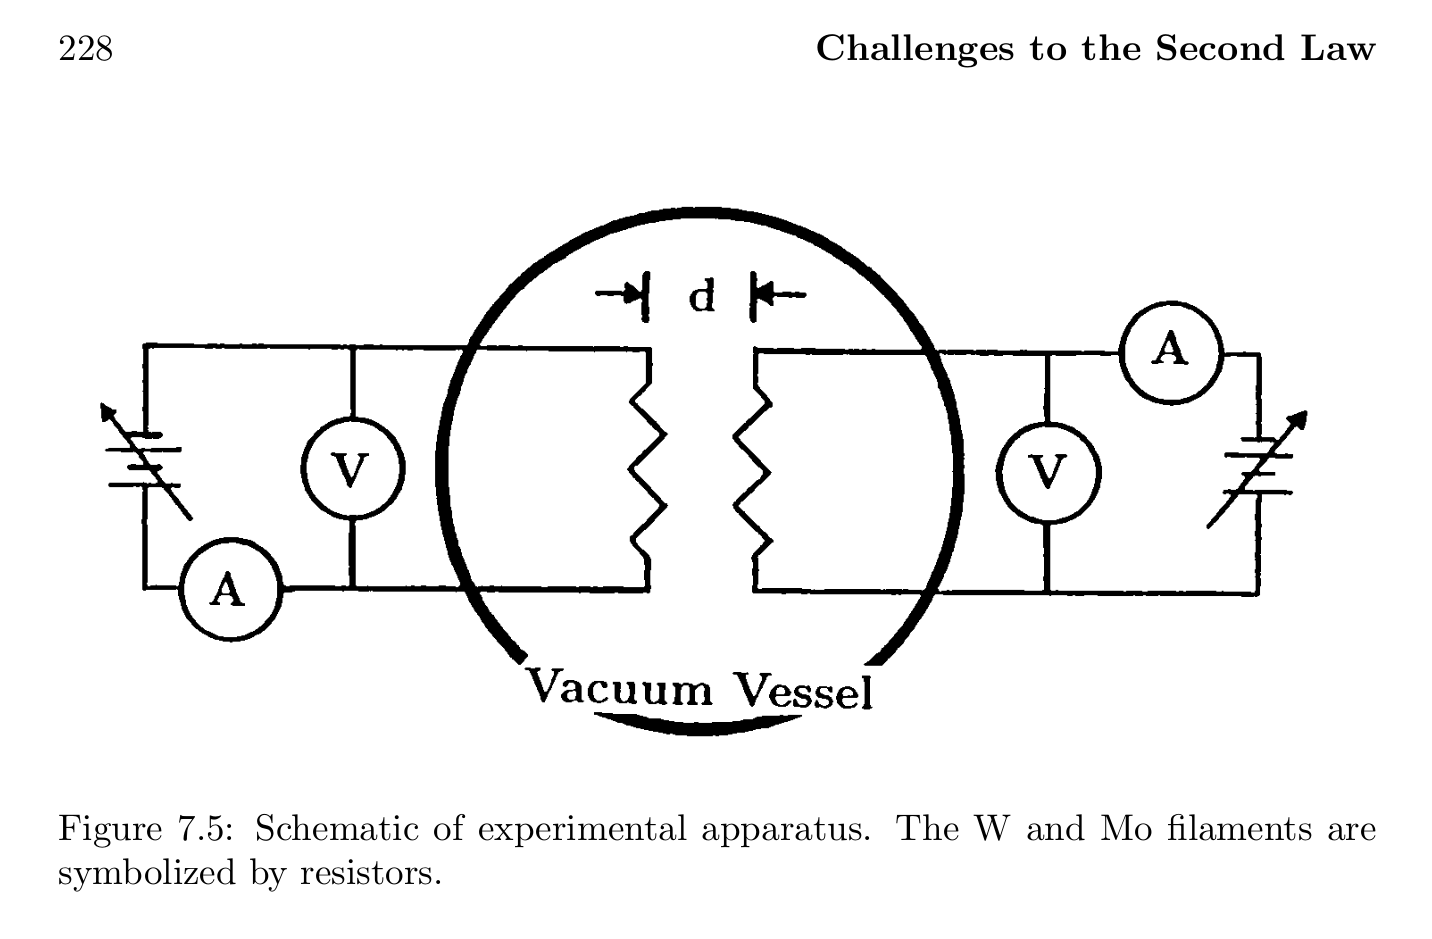
\includegraphics[width=0.7\textwidth]{Capek_fig7.5.png}
\caption{Схема осмоса в нанопорах (Capek et al.)}
\label{fig:capek5}
\end{figure}

\begin{figure}[htbp]
\centering
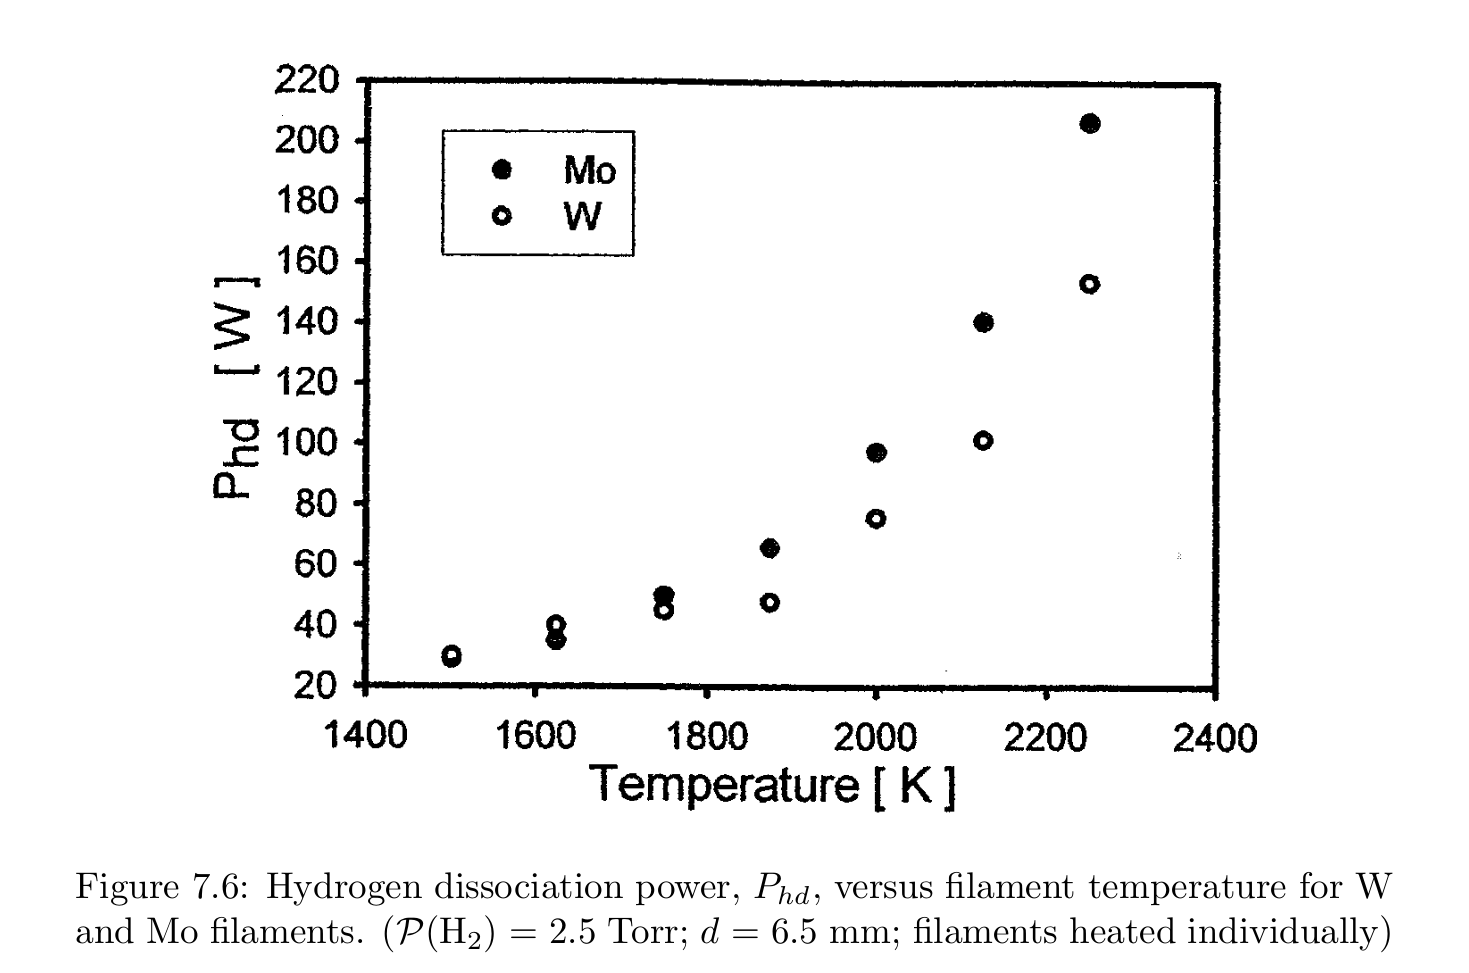
\includegraphics[width=0.7\textwidth]{Capek_fig7.6.png}
\caption{Зависимость потока от градиента давления (Capek et al.)}
\label{fig:capek6}
\end{figure}

\begin{figure}[htbp]
\centering
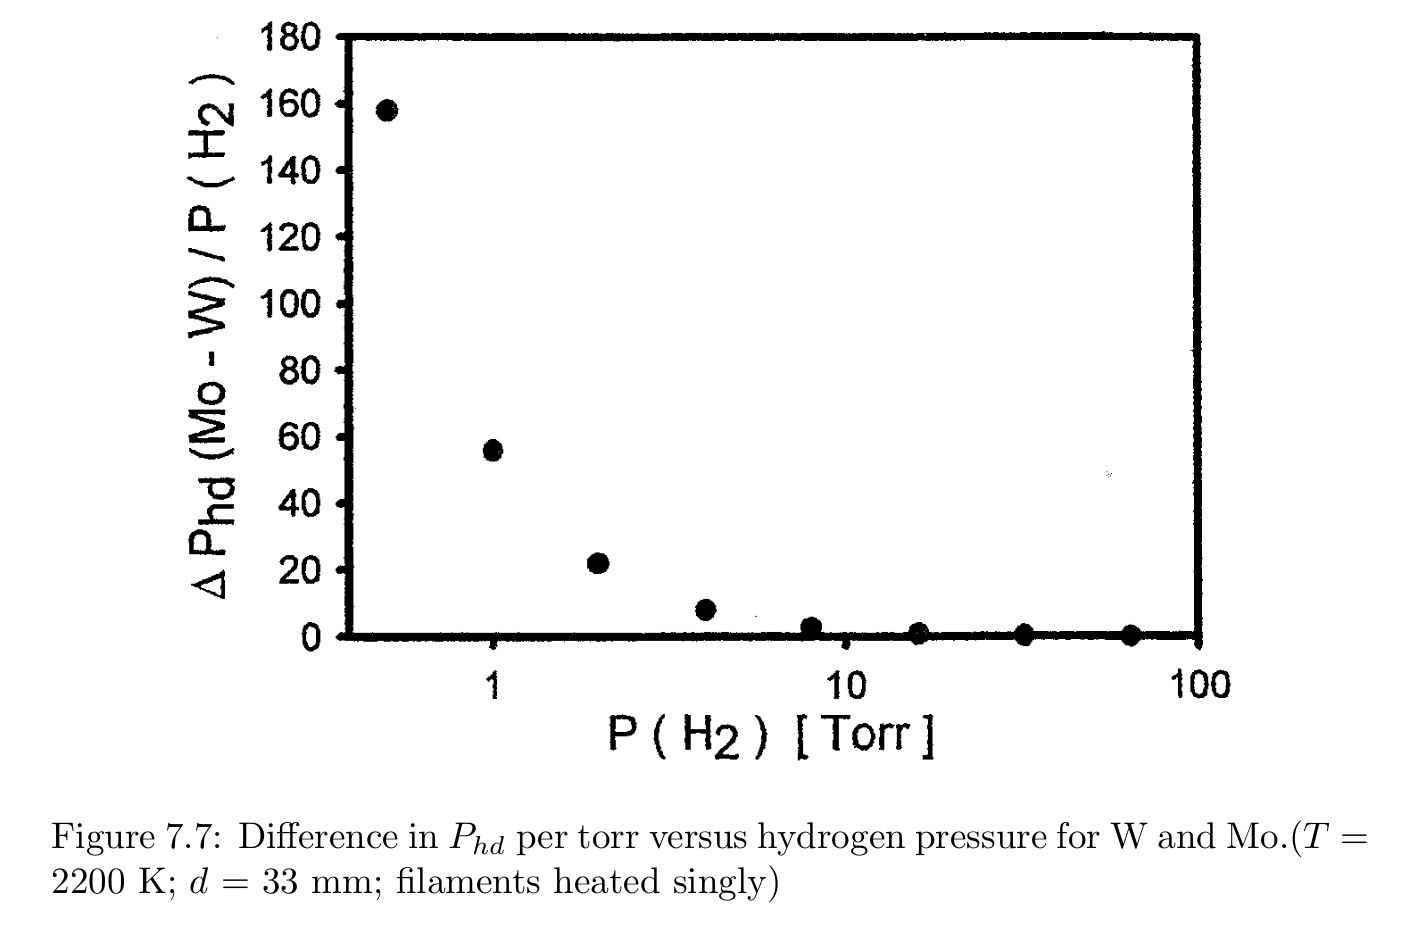
\includegraphics[width=0.7\textwidth]{Capek_fig7.7.png}
\caption{Температурная зависимость проницаемости (Capek et al.)}
\label{fig:capek7}
\end{figure}

\section{Как оценить ожидаемую мощность}

Какие нужно найти экспериментальные данные, чтобы попытаться оценить ожидаемую мощность никель-водородного или аналогичного ему биметалл-водородного кольцара.

\section{Метод оценки на основании изотерм адсорбции}

Нужно найти литературные данные о зависимости давления водорода, находящегося в равновесных условиях с поверхностью того или иного $hkl$ среза монокристалла металла, в зависимости от степени насыщения поверхности этого металла водородом (на английском это называется coverage, adsorbate concentration и обозначается как большая буква $\Theta_H$, имеет безразмерную величину и встречающиеся на практике величины от 0 до 2).

\section{Метод оценки на основании данных о кинетике адсорбции}

Что важно учесть -- поверхности могут отличаться первым или вторым порядком кинетики процессов адсорбции или десорбции.

\end{document}
